\documentclass[11pt,leqno]{article}
\usepackage[T1]{fontenc}
\usepackage[polish]{babel}
\usepackage[utf8]{inputenc}
\usepackage{a4wide}
\usepackage{amsmath}
\usepackage{graphicx}
\usepackage{algpseudocode}
\usepackage{algorithm}

\title{
  \textbf{Pracownia 2 z analizy numerycznej}\\
  \textit{Zadanie 20}
}
\author{Łukasz Hanuszczak}
\date{Wrocław, \today}

\begin{document}
\maketitle


\section{Wstęp}
Z reguły w zadaniu dotyczącym zagadnienia aproksymacji jednostajnej dana jest pewna kombinacja liniowa wielomianów ortogonalnych $p_i(x)$, przybliżająca funkcję:
\begin{equation} \label{eq:psum}
  f(x) \approx s(x) = \sum_{k = 0}^n w_i p_i(x)
\end{equation}
gdzie $p_i(x)$ spełniają zależność rekurencyjną:
\[ p_0(x) = a_0 \]
\begin{equation} \label{eq:prec}
p_1(x) = (a_1 x - b_1) p_0(x)
\end{equation}
\[ p_n(x) = (a_n x - b_n) p_{n - 1}(x) - c_n p_{n - 2} \text{, dla } k = 2, 3, \dots \]
dla pewnych ustalonych współczynników $a_0, \dots, a_n, b_1, \dots, b_n, c_1, \dots, c_n$.

Ważne jest więc aby wyliczać wartości $s(x)$ w sposób możliwie najszybszy i najdokładniejszy. W poniższym dokumencie opisane zostaną metody ewaluacji tego typu wielomianów, szczególnie na tak zwanym ,,algorytmie Clenshawa''.

Ponadto dzięki zapisaniu funkcji w postaci kombinacji liniowej wielomianów łatwo znaleźć wzór na $l$-tą pochodną:
\[
  f^l(x) \approx s^l(x) = \sum_{k = 0}^n w_i p_i^l(x)
\]

Przykładowo, wtedy wartości pierwszej pochodnej ciągów $p_i(x)$ spełniają podobną zależność rekurencyjną:
\[ p_0'(x) = 0 \]
\begin{equation} \label{eq:pprec}
p_1'(x) = (a_1 x - b_1) p_0'(x) + (a_1 x - b_1)' p_0(x) = a_1 p_0(x)
\end{equation}
\[ 
  p_k'(x)
  =
  ((a_k x - b_k) p_{k - 1}(x))' - (c_k p_{k - 2}(x))'
  =
  a_k p_{k - 1}(x) + (a_k x - b_k) p_{k - 1}'(x) - c_k p_{k - 2}'(x)
\]



\section{Podejście standardowe (Forsythe)}
Nietrudno wymyślić metodę obliczania wartości $s(x)$ wprost z definicji, bez korzystania z dość zawiłej relacji na kolejne współczynniki jak to ma miejsce w algorytmie Clenshawa. Jeżeli przez $s_k(x)$ oznaczona zostanie suma częściowa, tj.
\[ s_k(x) = \sum_{i = 0}^k w_i p_i(x) \]
to oczywiście $s(x) = s_n(x)$, z kolei z definicji sumy $s_k = s_{k - 1} + w_i p_i(x) $. Ponieważ $p_i(x)$ spełniają zależność rekurencyjną, to mając zapamiętane wartości $p_{i - 1}(x)$ i $p_{i - 2}(x)$ można wyliczyć w stałym czasie wartość $p_i$. Algorytm ma więc złożoność liniową i w każdym kroku wykonuje niewielką ilość trywialnych operacji arytmetycznych. W pseudokodzie metoda Forsythe'a prezentuje się następująco:

\begin{algorithmic}
\State $p_0 \gets a_0$
\State $p_1 \gets a_1 x - b_1 p_0$
\State $s_1 \gets w_0 p_0 + w_1 p_1$
\For {$i = 2 \to n$}
  \State $p_i \gets (a_i x - b_i) p_{i - 1} - c_i p_{i - 2}$
  \State $s_i \gets s_{i - 1} + w_i p_i$
\EndFor
\State \Return $s_n$
\end{algorithmic}


\subsection{Pochodne}
Bardzo łatwo rozszerzyć powyższą metodę do obliczania $s'(x)$ pierwszej pochodnej korzystając bezpośrednio z wzorów (\ref{eq:pprec}).

\begin{algorithmic}
\State $p_0 \gets a_0$, $p'_0 \gets 0$
\State $p_1 \gets a_1 x - b_1 p_0$, $p'_1 \gets a_1$
\State $s_1 \gets w_0 p'_0 + w_1 p'_1$
\For {$i = 2 \to n$}
  \State $p_i \gets (a_i x - b_i) p_{i - 1} - c_i p_{i - 2}$
  \State $p'_i \gets a_i p_{i - 1} + (a_i x - b_i) p'_{i - 1} - c_i p'_{i - 2}$
  \State $s_i \gets s_{i - 1} + w_i p_i'$
\EndFor
\State \Return $s_n$
\end{algorithmic}

Niestety, dla pochodnych wyższych rzędów zadanie znacznie się komplikuje. Można próbować wyprowadzać wzory, jednak wyliczanie dowolnej pochodnej tą metodą byłoby kompletnie nieefektywne.


\section{Algorythm Clenshawa}
\textit{Algorytm Clenshawa} pozornie wygląda na bardziej skomplikowany, a już na pewno mniej oczywisty. Najlepiej myśleć o nim jak o generalizacji schematu Hornera, który to jest jego specjalnym przypadkiem. Wystarczy wyliczyć pomocniczy ciąg wartości $B_i$, spełniających zależnosć
\[
  B_i = 0 \text{, dla } i > n
\]
\[
  B_i = w_i + (a_{i + 1} x - b_{i + 1}) B_{i + 1} - c_{i + 2} B_{i + 2}
  \text{, dla } 0 \leq i \leq n
\]

Mając ciąg wartości $B_i$ poszukiwaną wartość $s(x)$ można otrzymać z tożsamości
\[
  s(x) = a_0 B_0
\]

\subsection{Właściwości numeryczne}
Podobnie jak metoda Forsythe'a algorytm ma złożoność liniową. Jednak w każdym kroku algorytmu wykonywane jest jedno mnożenie mniej co pozwala prognozować, że algorytm będzie działał około 25\% szybciej. Pondato błędy wynikające z niedokładnej reprezentacji liczb w arytmetyce zmiennoprzecinkowej kumulują się wolniej. Zatem algorytm Clenshawa jest nie tylko szybszy ale też bardziej stabilny numerycznie.

\subsection{Dowód}
Dzięki prostym przekształceniom wzoru na $B_i$ można dojść do postaci:
\[
w_i = B_i - (a_{i + 1} x - b_{i + 1}) B_{i + 1} + c_{i + 2} B_{i + 2}
\]
Zatem
\[
  s(x)
=
  \sum_{k = 0}^n
    w_k p_k(x)
=
  \sum_{k = 0}^n
    (B_k - (a_{k + 1} x - b_{k + 1}) B_{k + 1} + c_{k + 2} B_{k + 2}) p_k(x)
=
\]
\[
=
  \sum_{k = 0}^n
    B_k p_k(x)
  -
  \sum_{k = 0}^n
    (a_{k + 1} x - b_{k + 1}) B_{k+1} p_k(x)
  +
  \sum_{k = 0}^n
    c_{k + 2} B_{k + 2} p_k(x)
=
\]
\[
=
  \sum_{k = 0}^n
    B_k p_k(x)
  -
  \sum_{k = 1}^{n + 1}
    (a_k x - b_k) B_k p_{k - 1}(x)
  +
  \sum_{k = 2}^{n + 2}
    c_k B_k p_{k - 2}(x)
\]
Ponieważ $B_{n + 1}$ oraz $B_{n + 2}$ są z definicji 0, to ostatnie elementy sumy drugiej i trzeciej znikają:
\[
  s(x)
=
  \sum_{k = 0}^n
    B_k p_k(x)
  -
  \sum_{k = 1}^n
    B_k p_{k - 1}(x) (a_k x - b_k)
  +
  \sum_{k = 2}^n
    B_k p_{k - 2}(x) c_k
=
\]
\[
\begin{split}
  \left(
  B_0 p_0(x) + B_1 p_1(x) + \sum_{k = 2}^n
    B_k p_k(x)
  \right)
  -
  \left(
  B_1 p_0(x) (a_1 x - b_1) + \sum_{k = 2}^n
    B_k p_{k - 1}(x) (a_k x - b_k)
  \right)
  +\\
  \sum_{k = 2}^n
    B_k p_{k - 2}(x) c_k
=
\end{split}
\]
\[
  B_0 p_0(x) + B_1 (p_1(x) - p_0(x) (a_1 x - b_1)) + \sum_{k = 2}^n
    \left(
    B_k \left(p_k(x) - p_{k - 1}(x) (a_k x - b_k) + p_{k - 2}(x) c_k\right)
    \right)
\]

Z rekurencyjnej definicji na $p_k$ wyrażenia $p_1(x) - p_0(x) (a_1 x - b_1)$ i $p_k(x) - p_{k - 1}(x) (a_k x - b_k) + p_{k - 2}(x) c_k$ są równe 0. W takim razie ostatecznie:

\[
  s(x) = B_0 p_0(x) = B_0 a_0
\]



\subsection{Pochodne (modyfikacja Smitha)}
Okazuje się, że powyższych algorytm daje się rozszerzyć także na obliczanie kombinacji liniowej pochodnych powyższych wielomianów.. Poniższego odkrycia dokonał w 1965 roku Francis J. Smith.

Niech $B_k$ tymi samymi pomocniczymi wartościami, wyliczonymi wcześniej dla zwykłego algorytmu Clenshawa. Wzór na $s'(x)$ można wyznaczyć podobnie jak to było w przypadku algorytmu Clenshawa:

\[
\begin{split}
  s'(x)
=
  \sum_{k = 0}^n w_k p_k'(x)
=
  \overbrace{w_0 p_0'(x)}^0 + \sum_{k = 1}^n w_k p_k'(x)
=\\=
  \sum_{k = 1}^n
    (B_k - (a_{k + 1} x - b_{k + 1}) B_{k + 1} + c_{k + 2} B_{k + 2}) p_k'(x)
=
\end{split}
\]
\[
=
  \sum_{k = 1}^n
    B_k p_k'(x)
  -
  \sum_{k = 1}^n
    (a_{k + 1} x - b_{k + 1}) B_{k + 1} p_k'(x)
  +
  \sum_{k = 1}^n
    c_{k + 2} B_{k + 2} p_k'(x)
=
\]
\[
=
  \sum_{k = 1}^n
    B_k p_k'(x)
  -
  \sum_{k = 2}^{n + 1}
    (a_k x - b_k) B_k p_{k - 1}'(x)
  +
  \sum_{k = 3}^{n + 2}
    c_k B_k p_{k - 2}'(x)
=
\]
\[
\begin{split}
=
  B_1 \overbrace{p_1'(x)}^{a_1 p_0(x)}
  +
  B_2 p_2'(x)
  +
  \sum_{k = 3}^n B_k p_k'(x)
  -
  (a_2 x - b_2) B_2 p_1'(x) - \sum_{k = 3}^n (a_k x - b_k) B_k p_{k - 1}'(x)
  +\\+
  \sum_{k = 3}^n
    c_k B_k p_{k - 2}'(x)
=
\end{split}
\]
\[
=
  B_1 a_1 p_0(x) + B_2 \left( \overbrace{
    p_2'(x) - (a_2 x - b_2) p_1'(x)
  }^{a_2(x) p_1(x)} \right)
  +
  \sum_{k = 3}^n
    B_k \overbrace{
      \left(p_k'(x) - (a_k x - b_k) p_{k - 1}' + c_k p_{k - 2}' \right)
    }^{a_k p_{k - 1} \text{na mocy (\ref{eq:pprec})}}
\]
\[
  s'(x) =  \sum_{k = 1}^n B_k a_k p_{k - 1}(x)
\]

W ten sposób poszukiwana wartość $s'(x)$ znowu jest kombinacją liniową wielomianów $p_i$, tym razem ze współczynnikami $B_k a_k$. To oznacza że zadanie sprowadzone zostało do tego samego problemu co wersja bez pochodnych, więc wystarczy użyć znanego już algorytmu Clenshawa.

Co więcej, na $s'(x)$ zapisanym w takiej formie można znowu użyć metody Smitha otrzymując $s''(x)$ w postaci kombinacji liniowej wielomianów ortogonalnych. Stosując ją po raz kolejny dostaje się $s'''(x)$ i tak dalej, stosując wariant Smitha algorytmu Clenshawa $l$ razy otrzymamuje się $s^l(x)$, co w przypadku metody Forsythe'a było niemożliwe (a przynajmniej dużo bardziej skomplikowane).

\section{Analiza}

\subsection{Wielomiany $I(x)$ i $J(x)$}
Treść zadania sugeruje przetestowanie algorytmu Clenshawa na wielomianach $I(x)$ oraz $J(x)$, które są liniową kombinacją wielomianów Czebyszewa, interpolujących funkcję $f$ odpowiednio węzłach:
\[
  t_k = \cos \frac{2k + 1}{2n + 2} \pi \; (k = 0, 1, \dots, n \; \text{dla $I(x)$})
\]
\[
  u_k = \cos \frac{k}{n} \pi \; (k = 1, \dots, n \; \text{dla $J(x)$})
\]
gdzie
\[
  I(x) = \sum_{i = 0}^n {}^{'}
    \frac{2}{n + 1} \left( \sum_{j = 0}^n f(t_j) T_i(t_j) \right) T_i(x)
\]
\[
  J(x) = \sum_{i = 0}^n {}^{''}
    \frac{2}{n} \left( \sum_{j = 0}^n {}^{''} f(u_j) T_j(u_i) \right) T_i(x)
\]
zaś $T_i(x)$ jest $i$-tym wielomianem Czebyszewa.

\subsubsection{Funkcja Rungego}
Funkcja Rungego jest klasycznym przykładem do testowania wielomianów interpolacyjnych ze względu na jej ,,destruktywne'' właściwości. W klasycznym przypadku wyraża się ona wzorem:
\[
  f(x) = \frac{1}{1 + 25x^2}
\]
Przy użyciu wyżej opisanego algorytmowi Smitha testowi poddana została także pierwsza pochodna funkcji Rungego, to jest:
\[
  f(x) = \frac{-50 x}{(1 + 25x^2)^2}
\]
Poniżej zaprezentowano wyniki dla interpolacji wielomianami $I(x)$ i $J(x)$ stopnia 10 i 100, dla większych $n$ wykresy liniowe stają się praktycznie nieczytelne.

Z zaprezentowanych i niezaprezentowanych wykresów wynika, że wielomiany $I(x)$ mają dużo mniej stabilną naturę niż wielomiany $J(x)$ co uwidacznia się szczególnie dla większych wartości $n$ na krańcach przedziałów.

\begin{center}
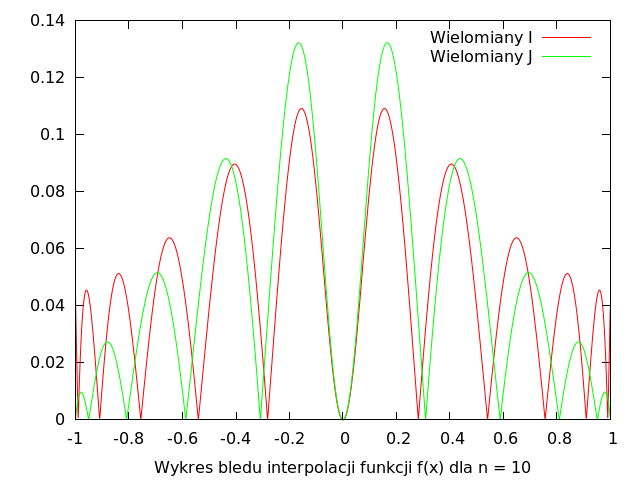
\includegraphics[scale=0.65,natwidth=640,natheight=480]{plot/runge10e.png}\\
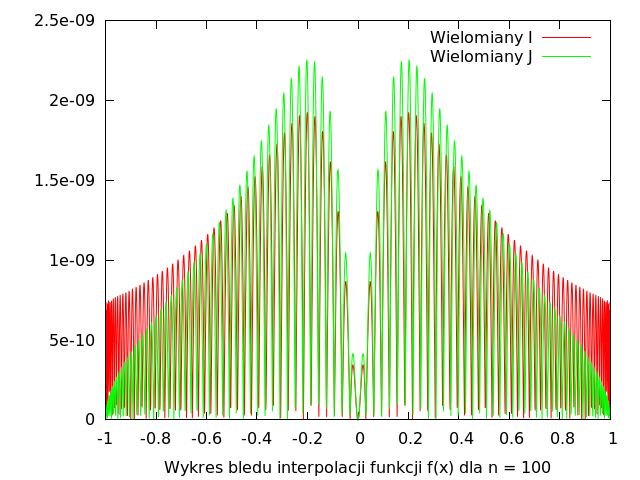
\includegraphics[scale=0.65,natwidth=640,natheight=480]{plot/runge100e.png}\\
\end{center}

\begin{center}
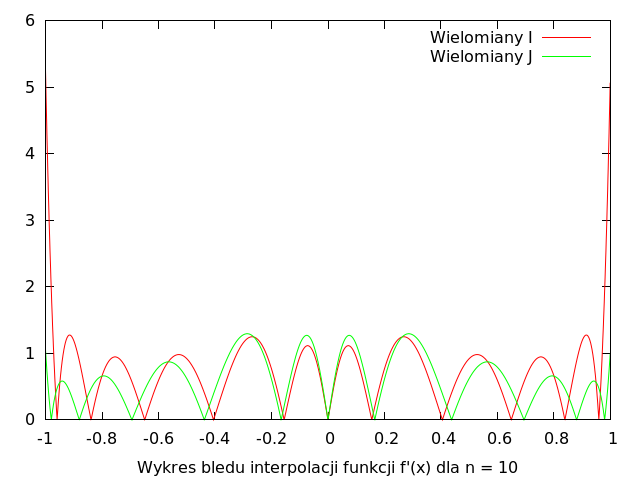
\includegraphics[scale=0.65,natwidth=640,natheight=480]{plot/runge10de.png}\\
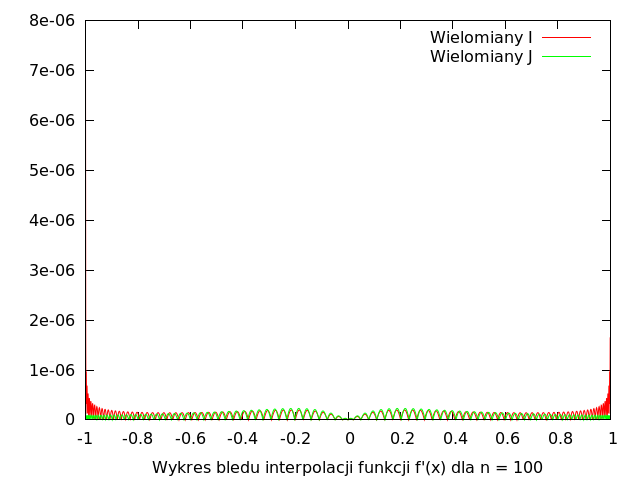
\includegraphics[scale=0.65,natwidth=640,natheight=480]{plot/runge100de.png}\\
\end{center}


\subsubsection{Funkcje $\sin$ i $\cos$}
Kolejnymi funkcjami, które poddane zostaną testowi są funkcje $\sin$ i $\cos$. Dla urozmaicenia, ta druga zostanie policzona jako pochodna tej pierwszej przy pomocy opisanej powyżej metody Smitha. Analogicznie jak poprzednio, zaprezentowano wykresu błędów dla $n = 10$ i $n = 100$.

\begin{center}
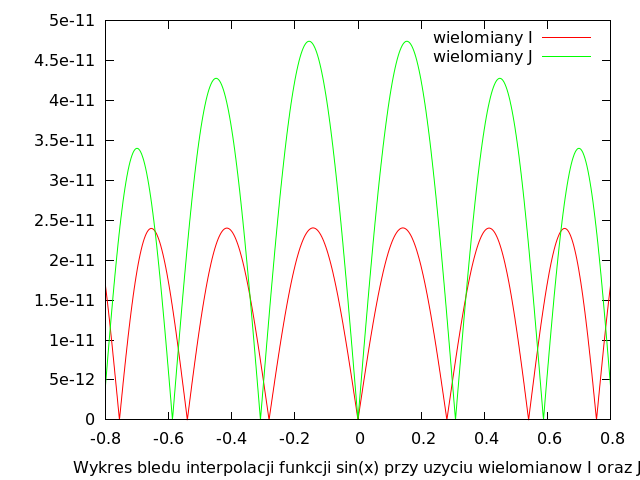
\includegraphics[scale=0.55,natwidth=640,natheight=480]{plot/sin10e.png}\\
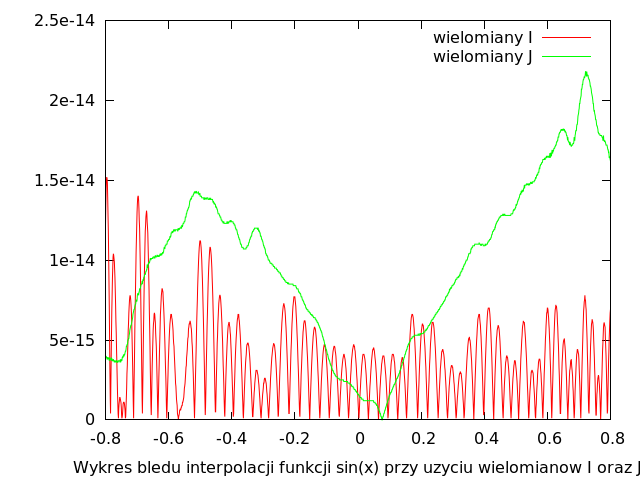
\includegraphics[scale=0.55,natwidth=640,natheight=480]{plot/sin100e.png}\\
\end{center}

\begin{center}
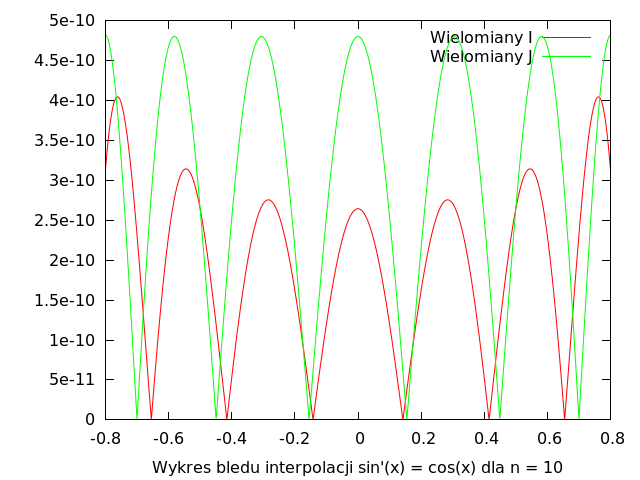
\includegraphics[scale=0.65,natwidth=640,natheight=480]{plot/cos10e.png}\\
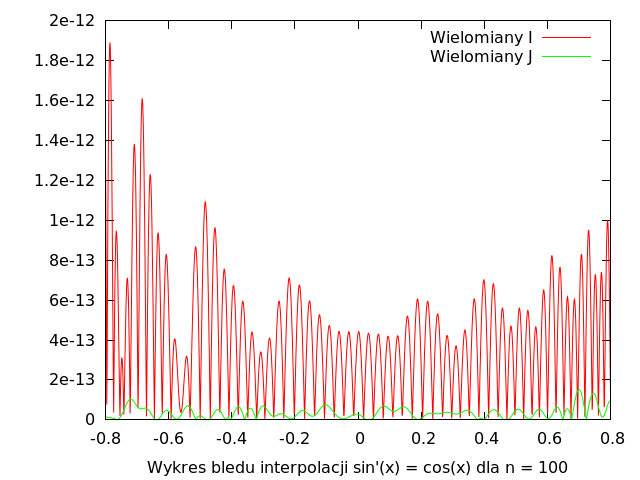
\includegraphics[scale=0.65,natwidth=640,natheight=480]{plot/cos100e.png}\\
\end{center}

Jak widać na powyższych wykresach w opozycji do testów z funkcją Rungego, tutaj mniej ,,stabilne'' są wielomiany $J(x)$. Można również zaobserowować, że aproksymacja funkcji $\cos$ przy pomocy pochodnej interpolowanego $\sin$ traci około 1 lub 2 najmniej znaczących cyfr w porównaniu do interpolowanego $\sin$.

\subsubsection{Wielomian}
Jak wiadomo interpolacja funkcji będącej wielomianem przy pomocy wielomianu powinna dać dokładnie ten sam wielomian (dla wielomianów odpowiedniego stopnia). Oczywiście w świecie analizy numerycznej wyniki ,,dokładne'' nie istnieją, zatem interpolacja wielomianu to bardzo dobre pole do badania błędów obliczeń. Losowo wybranym wielomianem, który będzie poddany analizie jest:
\[
  w(x) = 3 x^3 - 2 x^2 + 4 x = I(x) = J(x)
\]
Natomiast jego pochodna:
\[
  w'(x) = 9 x^2 - 4 x + 4 = I'(x) = J'(x)
\]
Tym razem jednak porównywane będą ze sobą błędy obliczeń produkowane przez algorytmy Clenshawa i Forsythe'a, więc pod uwagę brana będzie tylko interpolacja przy użyciu wielomianów $J(x)$.

\begin{center}
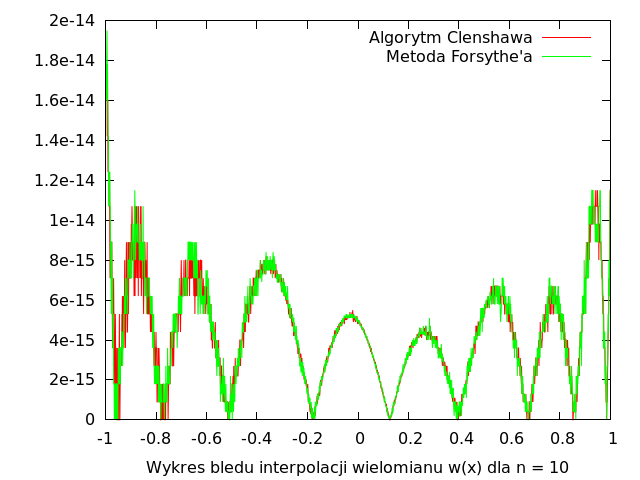
\includegraphics[scale=0.65,natwidth=640,natheight=480]{plot/poly10e.png}\\
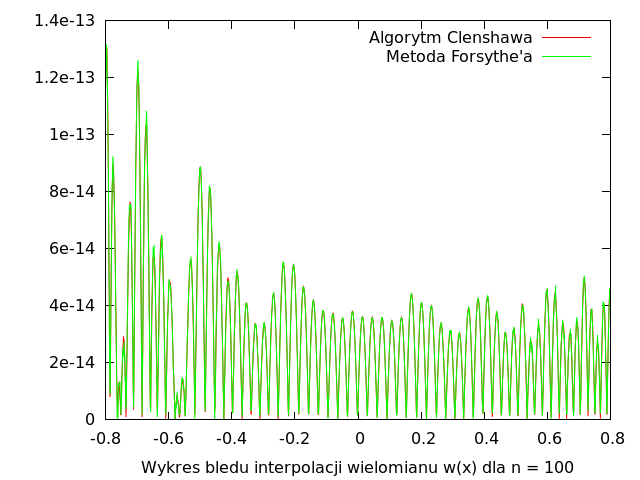
\includegraphics[scale=0.65,natwidth=640,natheight=480]{plot/poly100ezoom.png}\\
\end{center}

\begin{center}
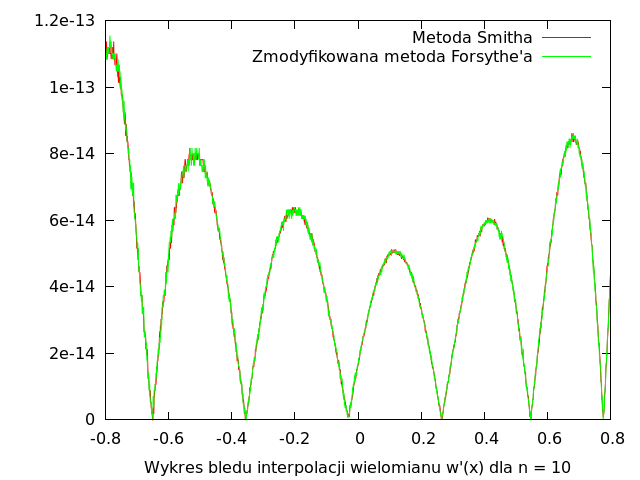
\includegraphics[scale=0.65,natwidth=640,natheight=480]{plot/poly10dezoom.png}\\
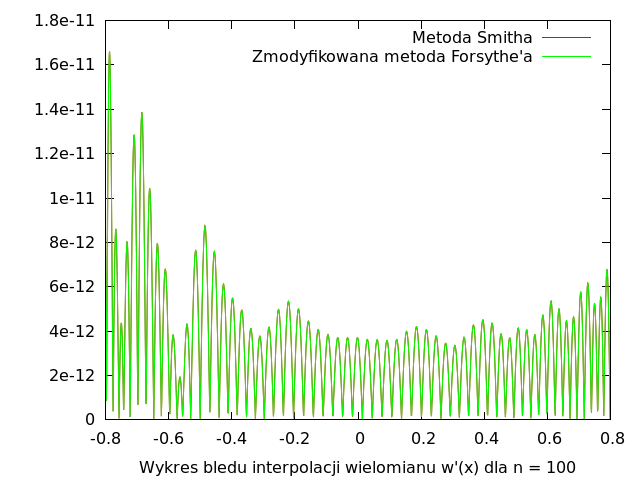
\includegraphics[scale=0.65,natwidth=640,natheight=480]{plot/poly100dezoom.png}\\
\end{center}

Z powyższych wykresów można wywnioskować, że obydwie metody dają niemal identyczne wyniki z minimalnie lepszymi, w większości przypadków, dla metody Clenshawa. Dla $n = 10$ błędy są na granicy precyzji arytmetyki mając około 1 niedokładnej cyfry. Gorzej jest natomiast dla $n = 100$ gdzie błąd zwiększa się do 2, 3 cyfr niedokładnych. Podobna sytuacja z pogorszeniem jakości wyniku wraz ze zwiększeniem $n$ ma miejsce w przypadku pochodnych.


\subsection{Inne testy}

\subsubsection{Wielomiany Lucasa}
Wielomiany Lucasa to wielomiany, generujące liczby Lucasa dla $x = 1$, zdefiniowane wzorem rekurencyjnym:
\[
L_0(x) = 2
\]
\[
L_1(x) = x
\]
\[
L_n(x) = x L_{n - 1}(x) + L_{n - 2}(x)
\]

To oznacza, że to obliczania ich kombinacji liniowej można użyć algorytmu Clenshawa. Przykładowo dla kombinacji liniowej:
\[
  s(x) = \sum_{i = 0}^8 (-1)^i L_i(x)
\]

W poniższej tabeli zostały zaprezentowane (prawie) dokładne wyniki $s(x)$ dla pewnych wartości $x$ oraz ich wyliczenia przy pomocy algorytmu Clenshawa ($\hat{s}(x)$).

\begin{center}
\begin{tabular}{ r || r | r }
  \hline
  x & $s(x)$ & $\hat{s}(x)$ \\
  \hline \hline
  $-\sqrt{3}$ & 970.1088913245535263 & 970.1088913245532694 \\
  $-\sqrt{2}$ & 401.7645019878171246 & 401.7645019878171979 \\
  $-1$        & 122.0000000000000000 & 122.0000000000000000 \\
  $0$         &  10.0000000000000000 & 10.0000000000000000  \\
  $1$         &  32.0000000000000000 & 32.0000000000000000  \\
  $\sqrt{2}$  & 130.2354980121828753 & 130.2354980121828874 \\
  $\sqrt{3}$  & 363.8911086754464736 & 363.8911086754462758
\end{tabular}
\end{center}


\subsubsection{Wielomiany Hermite'a}
Wielomiany Hermite'a to jeden z ważniejszych ciągów wielomianów ortogonalnych. Bez zbędnych szczegółów, spełniają one zależność rekurencyjną:
\[
  H_0(x) = 1
\]
\[
  H_1(x) = 2x
\]
\[
  H_n(x) = 2x H_{n - 1}(x) - 2(n - 1) H_{n - 2}(x)
\]
W tabeli poniżej zaprezentowano wyniki podobnie jak powyżej dla analogicznej kombinacji liniowej:
\[
  s(x) = \sum_{i = 0}^8 (-1)^i H_i(x)
\]

\begin{center}
\begin{tabular}{ r || r | r }
  \hline
  x & $s(x)$ & $\hat{s}(x)$ \\
  \hline \hline
  $-\sqrt{3}$ &  5242.848859344474566 &  5242.8488593444762955 \\
  $-\sqrt{2}$ &  4762.640835796065120 &  4762.6408357960681315 \\
  $-1$        & -1027.000000000000000 & -1027.0000000000000000 \\
  $0$         &  1571.000000000000000 &  1571.0000000000000000 \\
  $1$         & -1935.000000000000000 & -1935.0000000000000000 \\
  $\sqrt{2}$  &  3003.359164203934879 &  3003.3591642039364160 \\
  $\sqrt{3}$  &  6275.151140655525433 &  6275.1511406555227950 \\
\end{tabular}
\end{center}



\section{Podsumowanie}

Obydwa algorytmy faktycznie działają dając wyniki zbliżone do oczekiwanych dla testowanych danych (kombinacje liniowe wielomianów Lucasa, Hermite'a i Laguerre'a i Czebyszewa (wielomiany $I(x)$ i $J(x)$)).

Algorytm Clenshawa okazuje się być w praktycznym podejściu algorytmem niewiele, ale jednak, lepszym niż metoda standardowa (Forsythe), która z drugiej strony jest procedurą dużo bardziej intuicyjną. Testy wykazały niemal identyczne wyniki dla obydwu sposobów (działając w arytmetyce podwójnej precyzji), różniące się od siebie co najwyżej jedną lub dwoma najmniej znaczącymi cyframi.


\begin{thebibliography}{99}
\bibitem{WikiClenshaw} http://en.wikipedia.org/wiki/Clenshaw\_algorithm
\bibitem{WikiOrtho} http://en.wikipedia.org/wiki/Orthogonal\_polynomials
\bibitem{FJS} Francis J. Smith, An Algorithm for Summing Orthogonal Polynomial Series and their Derivatives with Applications to Curve-Fitting and Interpolation
\bibitem{Kincaid} David Kincaid, Werd Cheney, Analiza Numeryczna (2006)
\end{thebibliography}

\end{document}